% !TeX root = ../../manuscript.tex
\section{Results and discussion}

\subsection{Equilibration of the trajectories}
In this section, the equilibration of the protein during the various (cosolvent) \gls{md} trajectories is examined by plotting the \gls{rmsd} distance of the protein structure from its initial state throughout the simulated time.
On top of the usual task of selecting the equilibrated part of each trajectory to be considered for further analysis, these plots are useful to detect potential differences in the equilibration process between the traditional and the cosolvent trajectories.
On Figure \ref{fig:rmsd_equilib}, such plots obtained for the first replica of each solvent type are shown.
It is reassuring, that the protein structures seem to be well equilibrated after 50 ns of simulation time in all three cases.
The equilibration appears to be happening slightly faster in the benzene and especially in the phenol cosolvent trajectory than in water.
The equilibrated \gls{rmsd} values plotted on Figure \ref{fig:rmsd_equilib} are somewhat higher for the two cosolvent trajectories than in water.
This could indicate that the cosolvent probes have stabilised some conformations that are not often visited with water as solvent and that are farther from
the original protein conformation than those appearing frequently in water bas
ed simulations.
\begin{figure}
\centering
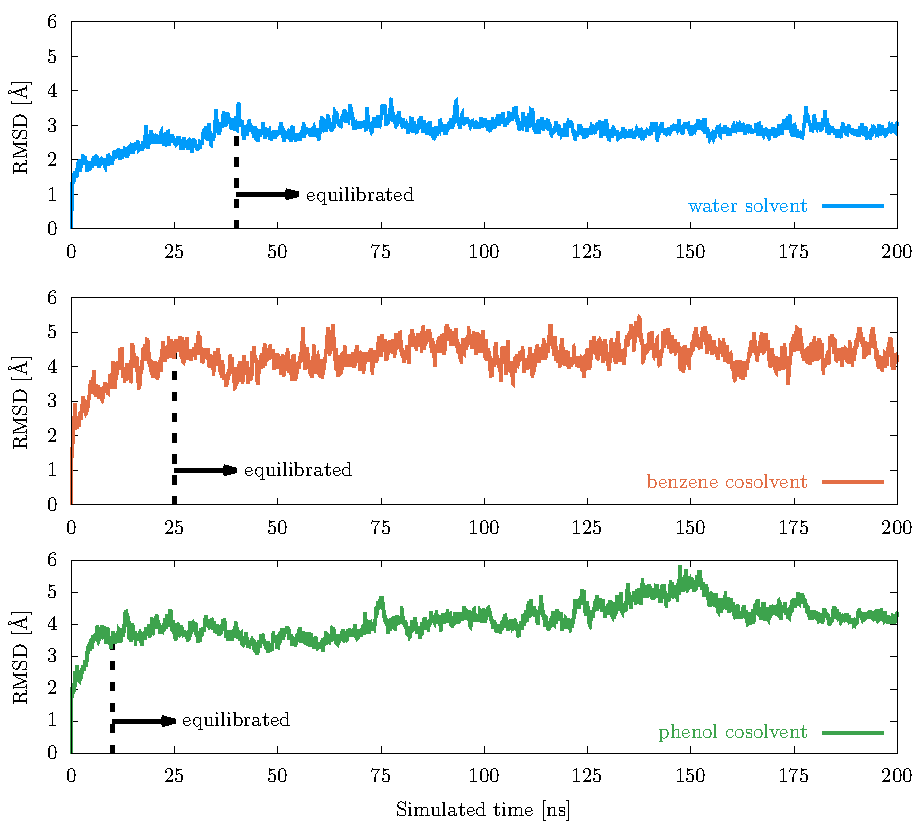
\includegraphics[width=\textwidth]{sections/results/images/rmsd_equilib/to_pdf/rmsd_equilib_to_pdf.pdf}
\caption{The evolution of the \gls{rmsd} distance of the protein from the starting conformation during the \gls{md} trajectories. The first replica for each solvent is plotted.}
\label{fig:rmsd_equilib}
\end{figure}

\subsection{Selecting representative protein conformations}
\newglossaryentry{dbi}{name={DBI},description={Davies--Bouldin index}}
\newglossaryentry{psf}{name={pSF},description={pseudo-F statistic}}
As mentioned in the Computational Details, the \texttt{dbscan} algorithm of \texttt{cpptraj} is used to perform the clustering of the trajectories.
The clustering is carried out separately for the three solvents, with the three replicas of each of them concatenated and treated as a single trajectory.
In order to carry out a successful clustering of the trajectories, first the $k$ and $\varepsilon$ parameters of the density based clustering algorithm have to be tuned.
On top of performing this tuning of the parameters, the effects of considering only the alpha carbon atoms for the \gls{rmsd} calculations instead of all heavy atoms of the protein are also evaluated.
Finally, possible redundancies in the set of representative protein structures are investigated.

The tuning of the parameters of the \texttt{dbscan} algorithm is performed by systematically varying the values for these parameters to see which combination yields the most optimal clustering.
% Additionally, clustering based only on the \gls{rmsd}s of alpha carbon atoms is compared with all heavy atom \gls{rmsd} clustering.
% The parameter $k$ is varied between four and seven, as the authors of \texttt{cpptraj} write in the User's Manual \cite{amberhub}, that values lower than four do not usually result in any improvements, while the value of of seven is already clearly inferior.
% The other parameter $\varepsilon$ is varied from 0.95 \AA{} to 1.3 \AA{} in the case of alpha carbon clustering, and from 1.3 \AA{} to 1.6 \AA{} when all heavy atoms are considered.
The computation of the \gls{rmsd} distances between all frames of a trajectory is much more demanding if on top of the alpha carbons, all other heavy atoms are considered as well.
To speed up these computations, the technique of sieving is utilised: only every other frame is considered explicitly during the clustering, the remaining frames are simply added to the cluster with the cluster representative most similar to them.
To measure the quality of the clustering four metrics are utilised.
Two of these have already been discussed, namely the \gls{dbi} and the \gls{psf}.
Since both of these scores are heavily influenced by the number of obtained clusters \cite{cluster_perf}, the comparison of their absolute values between different \gls{md} trajectories has limited meaning.
Instead, the trends arising in these metrics through the systematic variation of the clustering parameters can be interpreted to optimise these parameters.
At this point it is useful to reiterate, that low values of \gls{dbi} and high values of \gls{psf} are desirable.
The other two descriptors utilised to describe the quality of the clustering are the number of noise frames (frames not included in any cluster), and the number of clusters defined by the algorithm.
The number of noise frames should clearly be kept low to avoid missing any important conformations only because it is visited very rarely and is therefore considered an outlier by the algorithm.
Finally, while a high number of clusters is desirable as it can result in a wider variety of protein conformations, the computational limitations of performing explicit docking calculations to each representative conformation with thousands of ligands should be kept in mind.

On Figure \ref{fig:water_clustering_ca}, the descriptors of the water solvated trajectory clustering can be seen for the case when only the alpha carbons are considered during the \gls{rmsd} distance calculations.
As it can be seen from the figure, considering $\varepsilon$ values larger than 1.2 \AA{} leads to a single obtained cluster, for which the clustering descriptor metrics cannot provide a meaningful value.
% Considering the top two plots at first, it can be observed that the \gls{dbi} and \gls{psf} values are zero if $\varepsilon$ is greater than or equal to 1.2 \AA{}.
% The reason for this is that above this $\varepsilon$ value all frames of the trajectory are grouped into a single cluster, for which these descriptors cannot provide a meaningful value.
Since a single cluster is clearly not ideal, these large $\varepsilon$ values do not need to be considered during the search for the optimal parameters.
Focusing instead on parameter $k$, the most significant differences between the different values for this parameter can be discovered on the \gls{psf} plot.
Here, the curves with $k$= 4 or 6, reaching their peak at $\varepsilon$=1.1 \AA{}, are clearly superior to the other two.
% The curve corresponding to $k=7$ is somewhat of an outlier on this graph, with its peak \gls{psf} at $\varepsilon$=1.15 \AA{} instead of 1.1 \AA{}.
On the \gls{dbi} plot, the variation of $k$ has much more limited effects.
In fact, all curves are more or less constant if $\varepsilon$ is smaller than or equal to 1.1 \AA{}, at which point the \gls{dbi} values drop rapidly and become zero at 1.2 \AA{}.
Considering that $\varepsilon$=1.1 \AA{} is the point at which the \gls{dbi} values start decreasing, it is reasonable to assume that it is at this point that some significant changes are occurring in the way the clusters are defined.
Together with the fact that $\varepsilon$=1.1 \AA{} provides clusterings with the best \gls{psf} values, this observation makes this value of $\varepsilon$, together with $k$=4 a promising candidate to be the optimal choice.
Further advantages of this choice can be seen by looking at the bottom two plots of the figure: the number of noise frames stay below 2 \%, while a reasonable number of clusters (thirteen) is obtained.
The thirteen clusters resulting in thirteen representative protein conformations is deemed suitable both because docking to these conformations represents a manageable computational challenge, and because similar numbers of clusters have been reported in the literature for comparable \gls{md} trajectories \cite{24clusters-vina,clusters_vina2}.
% By looking at the bottom two plots of Figure \ref{fig:water_clustering_ca}, the number of noise frames and number of clusters can be observed.
% On these plots one can find further advantages of the $\varepsilon$=1.1 \AA{} choice.
% These are that the number of noise frames start their rapid increase only at slightly smaller epsilon values, and that a reasonable number of clusters, thirteen, are obtained for this value.
\begin{figure}
\centering
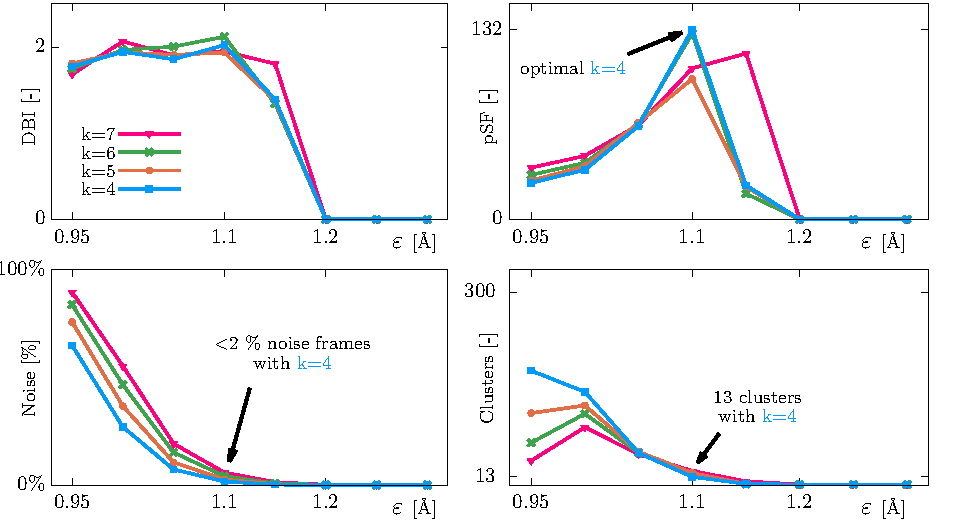
\includegraphics[width=\textwidth]{sections/results/images/water_clustering_ca/to_pdf/water_clustering_ca_to_pdf.pdf}
\caption{Plots of the clustering descriptors utilised for the tuning of the  \texttt{dbscan} parameters.
The descriptors were obtained by clustering the \gls{md} trajectory with water as the solvent and considering only the alpha carbon atoms for the \gls{rmsd} calculations.
The $\varepsilon$ parameter in units of \aa{}ngstr\"oms are shown on the horizontal axes in all cases, while on the vertical axes the various unitless descriptors are shown.
From the top left in clockwise direction: the Davies--Bouldin index, the pseudo-F statistic, the number of clusters and the number of noise frames are shown.}
\label{fig:water_clustering_ca}
\end{figure}

As a comparison, similar descriptors are calculated for the clusterings when all heavy atoms are considered during the \gls{rmsd} calculations.
The trends shown observed in this case look very similar to those discussed when only the alpha carbons are considered, therefore these plots are omitted.
The only notable difference is that significantly larger $\varepsilon$ values are needed to obtain similar results as in the case when only the alpha carbons are considered.
This phenomena can be explained if higher mobility is assumed for the non-backbone heavy atoms of the protein in comparison to the alpha carbons.
% A further difference is that now the curve corresponding to the $k$ value of four produces the best \gls{psf} values by a large margin instead of being only slightly better in the case of alpha carbon clustering.
% The number of noise frames is even more favorable in this case, however the ratio of noise frames is already negligible for reasonable values of $k$ and $\varepsilon$, when only the alpha carbons are considered.
% On the contrary, the number of defined clusters is far too low if all heavy atoms are considered, with only two clusters at $\varepsilon$=1.45 \AA{} and $k$=4.
Since no clear advantage of the all heavy atom clustering is found, the significantly increased computational costs of considering much more atoms for the \gls{rmsd} calculations make this type of clustering an inferior option compared to considering only the alpha carbons.

The performance of the clustering algorithm is also examined on the benzene cosolvent trajectory, with only the alpha carbons considered for clustering, to investigate any potential differences in the quality of the clustering due to the presence of cosolvent probes during the simulation.
The same descriptors as in the case of the water solvated trajectory are plotted on Figure \ref{fig:benzene_clustering_ca}.
Contrary to the water trajectory, in this case the number of clusters does not decrease to a single one at higher $\varepsilon$ values but instead is saturated at three.
As a consequence, the \gls{dbi} and \gls{psf} values on the top graphs do not vanish for these values of $\varepsilon$.
Instead, a sudden shift can be observed between $\varepsilon$=1.0 \AA{} and 1.1 \AA{} for both metrics, while for values higher or lower than these, the curves are more or less constant.
The facts that this shift is occurring near $\varepsilon=1.1$ \AA{}, and that this value is already in the more favorable interval for both metric curves, highlight the attractiveness of choosing 1.1 \AA{} as the value of the $\varepsilon$ parameter.
The \gls{psf} value at $\varepsilon=1.1$ \AA{} of the curve associated with $k=4$ is again one of the best along with $k=5$.
The bottom two plots reveal no surprises: the number of noise frames is negligible with the parameter values being seriously considered, while the number of clusters stagnates around the reasonable value of three and increases sharply only for $\varepsilon$ values less than 1.0 \AA{}.
Similar plots have been created for the trajectory with phenol as the cosolvent, however it showed very similar characteristics as this one, therefore it is not displayed here.
To summarise, the clustering parameters values of $\varepsilon$ = 1.1 \AA{} and $k$=4 prove to be ideal ideal choices, as they result in a clustering that is suitable for our purposes for all types of trajectories considered.
The resulting clustering yielded 19 total representative protein conformations (13 from the water, 3 from the benzene and 3 from the phenol trajectories), which were utilized during the subsequent ensemble docking calculations.
\begin{figure}
\centering
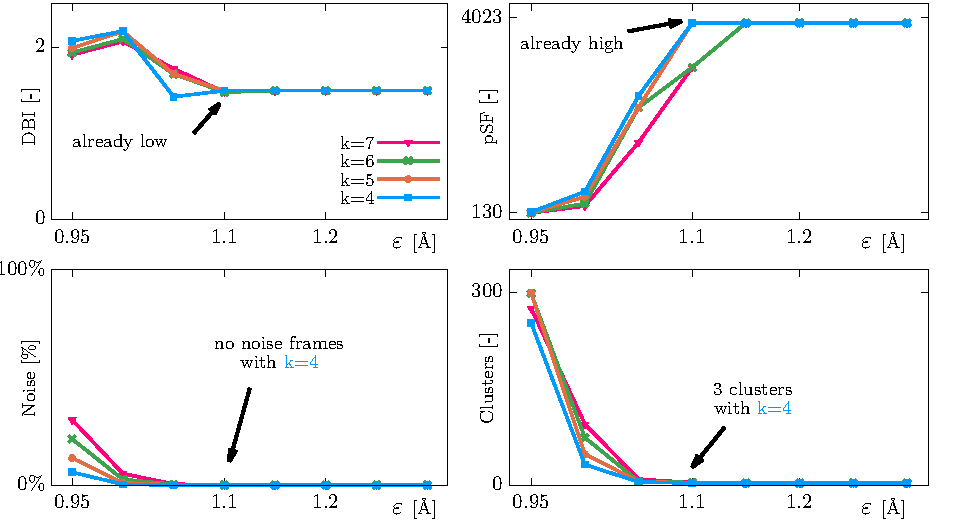
\includegraphics[width=\textwidth]{sections/results/images/benzene_clustering_ca/to_pdf/benzene_clustering_ca_to_pdf.pdf}
\caption{Plots of the clustering descriptors utilised for the tuning of the  \texttt{dbscan} parameters.
The descriptors were obtained by clustering the \gls{md} trajectory with benzene as the cosolvent and considering only the alpha carbon atoms for the \gls{rmsd} calculations.
The $\varepsilon$ parameter in units of \aa{}ngstr\"oms are shown on the horizontal axes in all cases, while on the vertical axes the various unitless descriptors are shown.
From the top left in clockwise direction: the Davies--Bouldin index, the pseudo-F statistic, the number of clusters and the number of noise frames are shown.}
\label{fig:benzene_clustering_ca}
\end{figure}

Since the clustering of the trajectories obtained with different solvents is carried out independently from each other, it is possible that some cluster representatives coming from different trajectories are quite similar to each other.
This redundancy would clearly not be optimal as it increases the computational requirements of the ensemble docking calculations without providing much additional information.
However, it is expected that the trajectories calculated with different cosolvents visit considerably different protein conformations and therefore significant redundancies between conformations coming from different solvents would be surprising.
Nonetheless, this potential redundancy is worth investigating as its presence could indicate that the cosolvent simulations are not performing as expected.
To this end, another clustering is performed utilising the parameters selected in the previous section, but with all trajectories considered at once.
This clustering yields 18 cluster representative structures which is only marginally less than the 19 obtained with the original clustering scheme.
The fact that the clustering algorithm cannot merge many clusters coming from different solvent trajectories, thus returns a similar number of clusters as when the trajectories are considered individually, signals that these trajectories indeed visit markedly different conformations.

To further confirm the assumption that conformations coming from trajectories with different solvents are more dissimilar to each other than conformations coming from the same trajectory, the \gls{rmsd} distances between all cluster representatives are calculated.
More specifically, the 19 representative protein conformations obtained in the previous section are taken, and \gls{rmsd} values between all possible pairs formed from them are calculated, considering only their alpha carbons.
By looking at the distribution of these \gls{rmsd} values for conformation pairs obtained from the same or from different \gls{md} trajectories, one can compare the intra- and intertrajectory similarity of protein conformations.
On Figure \ref{fig:clusterrep_distances}, one can observe this data, grouped by the solvent pairs from which the protein conformations are obtained.
The various curves on this plot represent the frequencies with which some \gls{rmsd} value is found among the distances calculated between cluster representatives of the two given solvents.
% For example the blue curve represents the distribution of the \gls{rmsd} distances between cluster representatives coming from the water solvent trajectory, while the yellow dashed curve represents this distribution measure between the representatives of the water and benzene trajectories.
The most noticeable feature of this graph is that the intratrajectory distances are noticeably smaller than the intertrajectory ones, with the solid curves being to the left of the dashed ones.
There is only a single outlier benzene conformation, which is quite dissimilar to all other cluster representatives coming from this trajectory.
To summarise, the data represented on this graph validates our assumption that the cosolvent trajectories visit conformations that are distinct from those visited by the traditional \gls{md} simulation with water as the solvent.
\begin{figure}
\centering
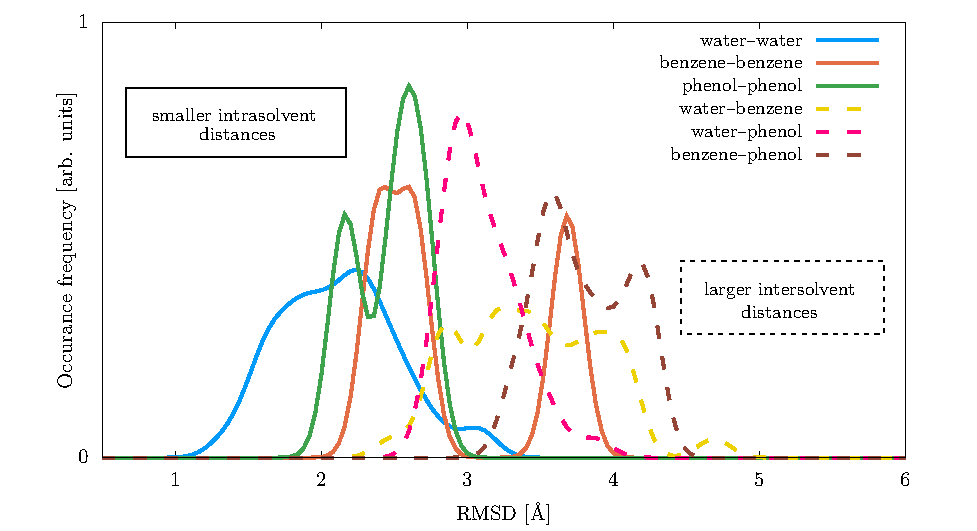
\includegraphics[width=\textwidth]{sections/results/images/clusterrep_distances/to_pdf/clusterrep_distances_to_pdf.pdf}
\caption{Plots of the clustering descriptors utilised for the tuning of the  \texttt{dbscan} parameters.
The descriptors were obtained by clustering the \gls{md} trajectory with benzene as the cosolvent and considering only the alpha carbon atoms for the \gls{rmsd} calculations.
The $\varepsilon$ parameter in units of \aa{}ngstr\"oms are shown on the horizontal axes in all cases, while on the vertical axes the various unitless descriptors are shown.
From the top left in clockwise direction: the Davies--Bouldin index, the pseudo-F statistic, the number of clusters and the number of noise frames are shown.}
\label{fig:benzene_clustering_ca}
\end{figure}
